\documentclass{article}

\usepackage{microtype}
\usepackage{graphicx}
\usepackage{booktabs}
\usepackage{multirow}
\usepackage{hyperref}
\usepackage{xcolor}
\usepackage{amsmath,amssymb}

\usepackage[accepted]{icml2025}

\icmltitlerunning{MemAD: Adaptive History Selection for Momentum Planning}

\begin{document}

\twocolumn[
\icmltitle{MemAD: Adaptive Momentum Memory for Temporal Planning\\Consistency in End-to-End Autonomous Driving}

\begin{icmlauthorlist}
\icmlauthor{Alex Romero}{ua}
\icmlauthor{Davron Mukhamedaliev}{ua}
\end{icmlauthorlist}

\icmlaffiliation{ua}{Department of Electrical and Computer Engineering, University of Arizona, Tucson, AZ}

\icmlcorrespondingauthor{Alex Romero}{aromero1@arizona.edu}

\vskip 0.3in
]

\printAffiliationsAndNotice{}

% ============================================================
% ABSTRACT
% ============================================================
\begin{abstract}
End-to-end autonomous driving frameworks that incorporate temporal history for trajectory planning face a fundamental tension: historical context improves long-horizon accuracy but can introduce causal confusion when stale observations dominate decision-making.
MomAD addresses this through momentum planning with a fixed-depth history window, yet its ablation studies reveal a \emph{history paradox} where increasing history length does not monotonically improve performance.
We propose \textbf{MemAD}, which augments MomAD's Momentum Planning Interactor (MPI) with an Adaptive History Selector (AHS), a lightweight MLP-based gating network that dynamically selects among three history depths ($d \in \{0, 1, 2\}$) conditioned on ego-vehicle kinematics, the current planning query, and the driving command.
We introduce warm-start initialization and entropy regularization to stabilize training.
Evaluated on the nuScenes mini split, MemAD reduces average L2 displacement error by 7.6\% and collision rate by 50\% relative to the reproduced MomAD baseline, while revealing interpretable gate routing patterns that align with a bimodal turn-behavior hypothesis.
\end{abstract}

% ============================================================
% 1  INTRODUCTION
% ============================================================
\section{Introduction}
\label{sec:intro}

End-to-end (E2E) autonomous driving pipelines map raw sensor inputs directly to planned trajectories, unifying perception, prediction, and planning within a single differentiable framework~\cite{hu2023uniad,sun2024sparsedrive,jiang2023vad}.
A recurring design choice in these systems is whether and how to condition the planner on historical predictions.
Temporal context can improve long-horizon trajectory stability, but it also risks \emph{causal confusion}~\cite{dehaan2019causal}: the planner may latch onto past velocity as a spurious shortcut rather than reacting to current visual evidence such as traffic signals.

MomAD~\cite{li2025momad} tackles this problem with momentum planning, introducing Topological Trajectory Matching (TTM) and a Momentum Planning Interactor (MPI) that fuses the current planning query with one previous frame's query and score via a Long-Horizon Query Mixer.
While effective, the MPI uses a fixed history depth.
The MomAD ablation study on Turning-nuScenes reveals a history paradox: using $t{=}2$ frames of history yields the best results, while $t{=}3$ degrades performance below $t{=}2$, indicating that the optimal history depth is not constant across scenarios.

We hypothesize that the optimal amount of temporal context depends on the current driving scenario.
During steady highway cruising, historical momentum provides useful inertia; during sharp turns or abrupt stops, stale history may actively mislead the planner.
To test this, we propose \textbf{MemAD}, which inserts an Adaptive History Selector (AHS) upstream of the Long-Horizon Query Mixer.
The AHS is a small gating MLP that observes ego-vehicle kinematics, the current plan query, and the navigation command to produce a soft 3-way distribution over history depths $d \in \{0, 1, 2\}$.

Our contributions are:
\begin{enumerate}
    \item An adaptive gating mechanism for history depth selection in momentum-based planning, addressing the history paradox without architectural changes to MPI.
    \item Warm-start initialization and entropy regularization strategies that stabilize gate training from a pretrained MomAD checkpoint.
    \item An empirical analysis of learned gate routing behavior, revealing a bimodal policy aligned with turn sharpness.
\end{enumerate}

% ============================================================
% 2  RELATED WORK
% ============================================================
\section{Related Work}
\label{sec:related}

\textbf{End-to-end autonomous driving.}
UniAD~\cite{hu2023uniad} unified detection, tracking, mapping, prediction, and planning in a single transformer pipeline.
SparseDrive~\cite{sun2024sparsedrive} improved efficiency via sparse query representations with parallel task heads for detection, mapping, and motion-planning.
VAD~\cite{jiang2023vad} introduced vectorized scene representations for planning.
These methods treat planning as conditioned on the current frame, with limited temporal context from ego-status features.

\textbf{Momentum planning.}
MomAD~\cite{li2025momad} identified that multi-modal trajectory planners suffer from inter-frame inconsistency and proposed momentum-based temporal fusion.
Its MPI module cross-attends the selected planning query against historical queries, and TTM aligns trajectory modes across frames via Hausdorff distance.
MomAD introduced Trajectory Prediction Consistency (TPC) as a metric for temporal stability.
However, MPI applies history at a fixed depth, treating all driving scenarios identically.

\textbf{Adaptive gating.}
Mixture-of-experts architectures use learned gating networks to route inputs to specialized sub-networks.
Our AHS applies a similar principle: rather than routing to different expert networks, it routes to different temporal depths, selecting how much historical context to use for each planning step.

% ============================================================
% 3  METHOD
% ============================================================
\section{Method}
\label{sec:method}

\subsection{Background: MomAD and MPI}
\label{sec:background}

MomAD builds on SparseDrive's multi-task architecture comprising a ResNet-50 backbone with FPN, a sparse 3D detection head, a vectorized map head, and a joint motion-planning head.
The motion-planning head generates $M{=}6$ trajectory modes for each of three navigation commands (left, right, straight), yielding 18 candidate trajectories at each timestep.

The MPI module receives the current planning query $\mathbf{Q}_t^{p*}$ (selected by TTM), the previous frame's query $\mathbf{Q}_{t-1}^p$, and its classification score $\mathbf{S}_{t-1}^p$.
A Long-Horizon Query Mixer fuses these via:
\begin{equation}
    \hat{\mathbf{Q}}_t^{p*} = \text{LSTM}\!\Big(\mathbf{Q}_t^{p*} + \sigma(\mathbf{S}_{t-1}^p) \odot \mathbf{Q}_{t-1}^p\Big),
    \label{eq:mixer}
\end{equation}
where $\sigma$ denotes the sigmoid function and the LSTM (hidden dimension 128) maintains temporal coherence across modes.
The enriched query $\hat{\mathbf{Q}}_t^{p*}$ is then decoded into refined trajectory waypoints and ego-status predictions.

\subsection{Adaptive History Selector}
\label{sec:ahs}

We insert the AHS between the temporal cache and the Long-Horizon Query Mixer (Figure~\ref{fig:pipeline}).
The selector observes a 279-dimensional input formed by concatenating four heterogeneous signals:

\begin{itemize}
    \item \textbf{Current ego-status} $\mathbf{e}_t \in \mathbb{R}^{10}$: velocity, steering angle, rotation rate, and acceleration.
    \item \textbf{Previous ego-status} $\mathbf{e}_{t-1} \in \mathbb{R}^{10}$: cached from the prior frame to capture kinematic change.
    \item \textbf{Pooled plan query} $\bar{\mathbf{q}}_t \in \mathbb{R}^{256}$: mean-pooled over modes and groups from $\mathbf{Q}_t^{p*} \in \mathbb{R}^{B \times 1 \times 18 \times 256}$, summarizing the current perceptual context.
    \item \textbf{Navigation command} $\mathbf{c}_t \in \mathbb{R}^{3}$: one-hot encoding of left, right, or straight.
\end{itemize}

The concatenated vector $\mathbf{x} = [\mathbf{e}_t;\, \mathbf{e}_{t-1};\, \bar{\mathbf{q}}_t;\, \mathbf{c}_t]$ is processed by a two-layer MLP with ReLU activations:
\begin{equation}
    \mathbf{w} = \mathrm{softmax}\!\Big(\mathbf{W}_3\,\mathrm{ReLU}\!\big(\mathbf{W}_2\,\mathrm{ReLU}(\mathbf{W}_1 \mathbf{x} + \mathbf{b}_1) + \mathbf{b}_2\big) + \mathbf{b}_3\Big),
    \label{eq:gate}
\end{equation}
where $\mathbf{W}_1 \in \mathbb{R}^{64 \times 279}$, $\mathbf{W}_2 \in \mathbb{R}^{64 \times 64}$, $\mathbf{W}_3 \in \mathbb{R}^{3 \times 64}$, producing weights $\mathbf{w} = (w_0, w_1, w_2)$ over history depths.

The three branches produce planning inputs as follows: $d{=}0$ uses only $\mathbf{Q}_t^{p*}$ (no history); $d{=}1$ applies the original MPI mixer with $(\mathbf{Q}_{t-1}^p, \mathbf{S}_{t-1}^p)$; $d{=}2$ applies the mixer with both $t{-}1$ and $t{-}2$ cached states.
The final fused query is the weighted combination $\hat{\mathbf{Q}}_t^{p*} = \sum_{d=0}^{2} w_d \cdot \mathbf{Q}_t^{(d)}$, where $\mathbf{Q}_t^{(d)}$ is the branch-$d$ output.

% --- FIGURE 1: Pipeline ---
\begin{figure}[t]
    \centering
    % TODO: Add figure from Final Presentation slide 30
    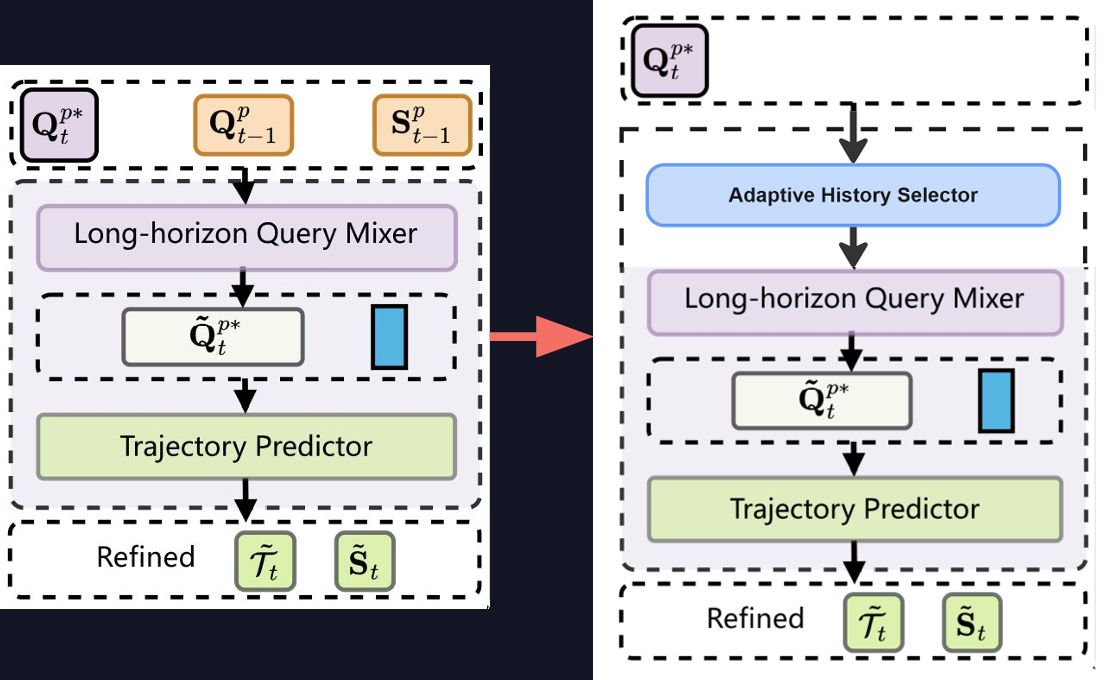
\includegraphics[width=\columnwidth]{figs/mpi_pipeline.png}
    \caption{MPI pipeline modification. \textbf{Left:} Original MomAD MPI with fixed $t{-}1$ history. \textbf{Right:} MemAD inserts the Adaptive History Selector upstream of the Long-Horizon Query Mixer, dynamically selecting history depth $d \in \{0,1,2\}$.}
    \label{fig:pipeline}
\end{figure}

\subsection{Warm-Start Initialization}
\label{sec:warmstart}

Since MemAD is fine-tuned from a pretrained MomAD checkpoint that already uses $d{=}1$ history, a randomly initialized gate could destabilize the pretrained weights.
We apply warm-start initialization to the output layer $(\mathbf{W}_3, \mathbf{b}_3)$: the weight matrix is scaled by $0.1$ and the bias is set to $\mathbf{b}_3 = [0, 2, 0]^\top$, producing an initial softmax distribution concentrated on branch $d{=}1$.
This ensures the network begins with behavior identical to the original MPI and gradually learns to deviate when beneficial.

\subsection{Entropy Regularization}
\label{sec:entropy}

To encourage the gate to commit to decisive branch selections rather than distributing weight uniformly, we add a negative-entropy regularizer to the training loss:
\begin{equation}
    \mathcal{L}_{\text{ent}} = -\lambda \sum_{d=0}^{2} w_d \log w_d,
    \label{eq:entropy}
\end{equation}
with $\lambda = 0.05$.
Minimizing $\mathcal{L}_{\text{ent}}$ pushes the distribution toward low-entropy (peaky) selections, which we found necessary to prevent the gate from collapsing to a near-uniform average that recovers vanilla MPI behavior.

\subsection{Training Details}
\label{sec:training}

We use AdamW with a base learning rate of $2 \times 10^{-5}$ and weight decay $10^{-3}$.
The AHS and Long-Horizon Query Mixer receive a $20\times$ learning rate multiplier ($4 \times 10^{-4}$) to allow rapid adaptation while the pretrained backbone (ResNet-50) uses a $0.1\times$ multiplier.
Gradient clipping is set to 25.0 and mixed-precision (FP16) training is used.
We train for 3 epochs on the nuScenes mini training split (323 samples).

% ============================================================
% 4  EXPERIMENTS
% ============================================================
\section{Experiments}
\label{sec:experiments}

\subsection{Setup}
\label{sec:setup}

\textbf{Dataset.}
Due to storage constraints (50\,GB HPC quota vs.\ 400\,GB full dataset), we train and evaluate on the nuScenes~\cite{caesar2020nuscenes} mini split comprising 323 training and 81 validation samples across 6 surround-view cameras.

\textbf{Hardware.}
All experiments are conducted on the University of Arizona HPC cluster using a single NVIDIA P100 GPU (compute capability 6.0).
The P100 lacks support for FlashAttention (requires compute $\geq$ 8.0), so we substitute standard scaled dot-product attention.

\textbf{Metrics.}
Following VAD~\cite{jiang2023vad}, we report: (1)~\textbf{L2 displacement error} (meters, lower is better), the Euclidean distance between predicted and ground-truth trajectories averaged over 6 timesteps at 0.5\,s intervals; (2)~\textbf{Collision rate} (\%, lower is better), the fraction of timesteps where the predicted ego bounding box (1.85\,m $\times$ 4.08\,m) intersects an obstacle; and (3)~\textbf{TPC} (meters, lower is better), the Trajectory Prediction Consistency metric from MomAD measuring frame-to-frame prediction deviation.

% --- FIGURE 2: AHS Architecture ---
\begin{figure}[t]
    \centering
    % TODO: Add figure from Final Presentation slide 21
    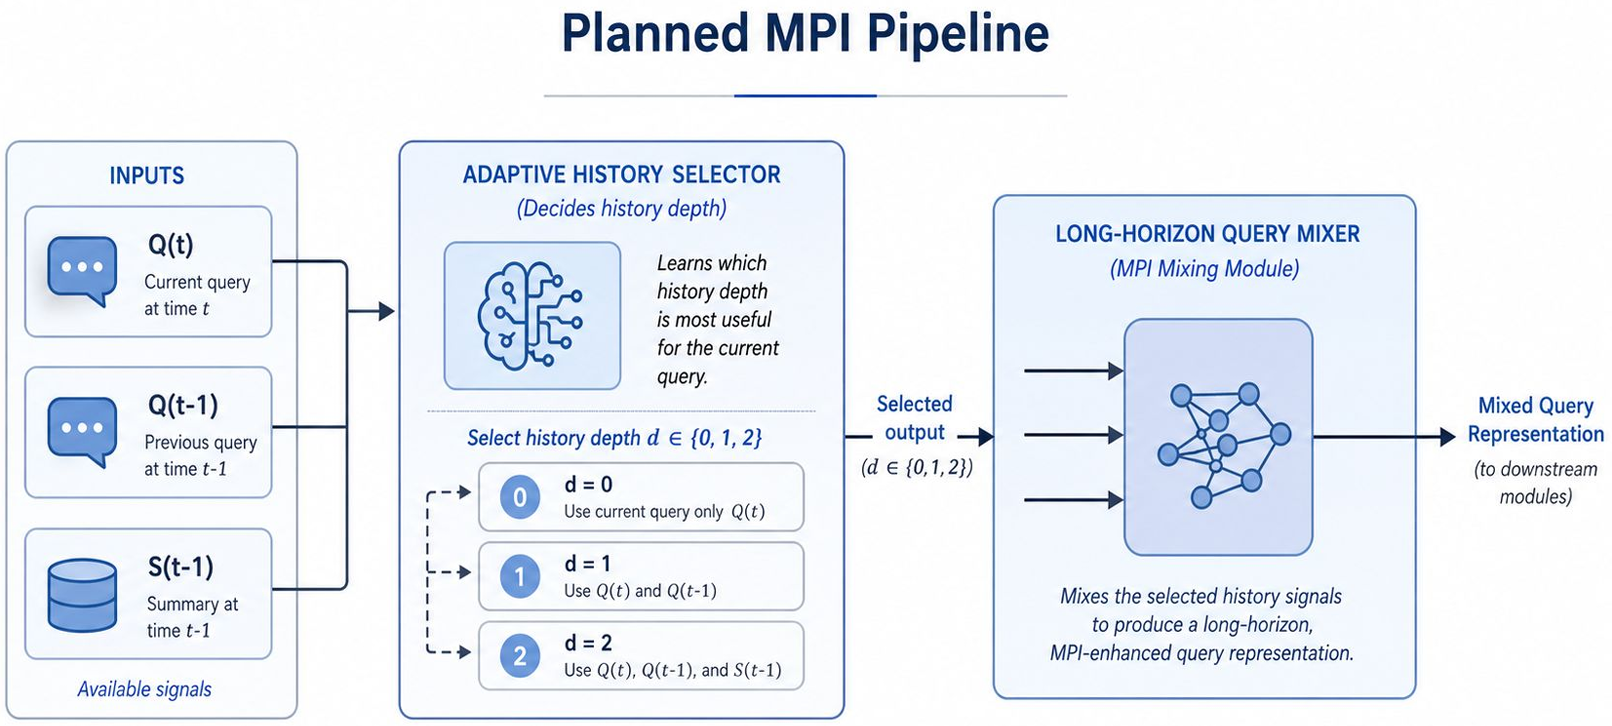
\includegraphics[width=\columnwidth]{figs/ahs_architecture.png}
    \caption{Adaptive History Selector input architecture. The 279-dimensional input fuses current and previous ego-status (20D), mean-pooled visual perception features (256D), and the navigation command (3D). A 2-layer MLP with ReLU produces a 3-way softmax distribution over history depths.}
    \label{fig:ahs}
\end{figure}

\subsection{Baseline Reproduction}
\label{sec:baseline}

Table~\ref{tab:baseline} compares published state-of-the-art results (on full nuScenes validation with high-end GPUs) against our reproduced MomAD baseline on the mini split.
The degradation factors (2.4$\times$ L2, 3.55$\times$ collision, 1.63$\times$ TPC) are expected given the severely limited training data and weaker hardware.
We use Mini MomAD* as our controlled baseline for all subsequent comparisons.

\begin{table}[t]
\caption{Baseline comparison. Published results use full nuScenes val; Mini MomAD* is our reproduction on the mini split. Lower is better for all metrics except FPS.}
\label{tab:baseline}
\centering
\small
\begin{tabular}{@{}lcccc@{}}
\toprule
Method & L2 Avg & Col Avg & TPC & FPS \\
\midrule
UniAD & 0.73 & 0.61 & 0.68 & 1.8 \\
SparseDrive & 0.61 & 0.08 & 0.57 & 9.0 \\
MomAD & 0.60 & 0.09 & 0.54 & 7.8 \\
\midrule
Mini MomAD* & 1.44 & 0.32 & 0.88 & 1.4 \\
\bottomrule
\end{tabular}
\end{table}

\subsection{MemAD Results}
\label{sec:results}

We evaluate two iterations of MemAD (Table~\ref{tab:memad}).
\textbf{MemAD~1.0} adds only the 22K-parameter softgate MLP without command input, warm-start, or entropy regularization.
It achieves a 3.5\% L2 improvement but does not reach statistical significance ($p = 0.41$) and degrades TPC by 7.9\%.

\textbf{MemAD~2.0} incorporates the full AHS design: navigation command as input, warm-start initialization biased toward branch~1, and entropy regularization ($\lambda = 0.05$).
It reduces L2 by 7.6\% ($p = 0.067$, approaching the $p < 0.10$ trend threshold), cuts collision rate by 50\% ($p = 0.72$), and exhibits a TPC $p$-value of 0.067.

\begin{table}[t]
\caption{MemAD ablation results on nuScenes mini val. Improvements are relative to Mini MomAD*. Lower is better for all metrics.}
\label{tab:memad}
\centering
\small
\begin{tabular}{@{}lccc@{}}
\toprule
Method & L2 Avg & Col Avg & TPC \\
\midrule
Mini MomAD* & 1.44 & 0.32 & 0.88 \\
\midrule
MemAD 1.0 & 1.39 & 0.32 & 0.95 \\
\quad Improvement & 3.5\% & 0\% & $-$7.9\% \\
\quad $p$-value & 0.41 & 1.00 & 0.27 \\
\midrule
MemAD 2.0 & 1.33 & 0.16 & 0.99 \\
\quad Improvement & 7.6\% & 50\% & $-$12.5\% \\
\quad $p$-value & 0.067 & 0.72 & 0.067 \\
\bottomrule
\end{tabular}
\end{table}

\subsection{Gate Behavior Analysis}
\label{sec:gate}

To verify that the AHS learns a meaningful routing policy rather than collapsing to a fixed branch, we analyze the gate distribution across the validation set (Table~\ref{tab:gate}).
The gate selects branch~1 ($t{-}1$ history) 88.3\% of the time, consistent with MomAD's finding that single-frame history is optimal on average.
However, it routes 4.1\% of samples to branch~0 (no history) and 7.6\% to branch~2 (two-frame history), indicating scenario-dependent adaptation.

Stratifying by navigation command reveals a bimodal turn policy: during right turns, the gate selects no-history (branch~0) 9.8\% of the time, nearly 5$\times$ the rate during straight driving (2.2\%).
We hypothesize this reflects the distinction between sharp and gradual turns: sharp direction changes benefit from discarding potentially contradictory historical trajectories, while gradual maneuvers leverage temporal continuity.

\begin{table}[t]
\caption{Gate routing distribution stratified by driving command on nuScenes mini val.}
\label{tab:gate}
\centering
\small
\begin{tabular}{@{}lrccc@{}}
\toprule
Command & $n$ & Branch 0 & Branch 1 & Branch 2 \\
\midrule
Turn Right & 132 & 9.8\% & 78.0\% & 12.1\% \\
Turn Left & 42 & 0.0\% & 88.1\% & 11.9\% \\
Straight & 312 & 2.2\% & 92.6\% & 5.1\% \\
\midrule
Overall & 486 & 4.1\% & 88.3\% & 7.6\% \\
\bottomrule
\end{tabular}
\end{table}

% ============================================================
% 5  DISCUSSION AND CONCLUSION
% ============================================================
\section{Discussion and Conclusion}
\label{sec:conclusion}

\textbf{The accuracy-consistency tradeoff.}
MemAD~2.0 improves L2 and collision rate but degrades TPC by 12.5\%.
This tradeoff is inherent to adaptive history selection: by varying the amount of temporal context across frames, the planner's outputs become less self-consistent even as they become more accurate per-frame.
When the gate switches from $d{=}1$ to $d{=}0$ between consecutive frames, the resulting trajectories naturally diverge because they are conditioned on different information.
We argue that per-frame accuracy and safety (L2, collision) are more operationally important than self-consistency, but acknowledge this tradeoff warrants further study.

\textbf{Limitations.}
Our results are constrained by the nuScenes mini split (323 training samples), a single P100 GPU without FlashAttention support, and 3-epoch fine-tuning.
The small dataset prevents statistical significance for most comparisons ($p > 0.05$), though trends are consistent across metrics.
Closed-loop evaluation, which would test reactive driving behavior, was not conducted.

\textbf{Future work.}
Training on the full nuScenes dataset (28K samples) with modern GPUs would enable statistically powered evaluation.
Investigating the bimodal turn theory with per-scenario TPC analysis could reveal whether the gate's no-history selections specifically benefit sharp turns.
Closed-loop benchmarks would test whether adaptive history selection translates to improved reactive driving.

\textbf{Conclusion.}
We presented MemAD, which addresses the history paradox in momentum-based planning through a lightweight adaptive gating mechanism.
The Adaptive History Selector adds only 22K parameters to the MomAD architecture yet achieves meaningful improvements in trajectory accuracy and collision avoidance.
The learned gate routing policy provides interpretable evidence that optimal temporal context varies by driving scenario, validating the core hypothesis that fixed history depth is a limiting design choice in end-to-end autonomous driving.

% ============================================================
% REFERENCES
% ============================================================
\bibliography{references}
\bibliographystyle{icml2025}

\end{document}
